\documentclass[a4]{article}
\usepackage[czech]{babel}
\usepackage[utf8]{inputenc}
\usepackage{listings}
\usepackage{hyperref}
\usepackage{color}
\usepackage{amsmath}
\usepackage{multicol}
\usepackage{titlesec}
\usepackage{graphicx}
\graphicspath{ {images/} }

\usepackage{relsize}

\setlength{\parskip}{1em}

\definecolor{dkgreen}{rgb}{0,0.6,0}
\definecolor{gray}{rgb}{0.5,0.5,0.5}
\definecolor{mauve}{rgb}{0.58,0,0.82}

\lstset{frame=tb,
  language=Octave,
  aboveskip=3mm,
  belowskip=3mm,
  showstringspaces=false,
  columns=flexible,
  basicstyle={\small\ttfamily},
  numbers=none,
  numberstyle=\tiny\color{gray},
  keywordstyle=\color{blue},
  commentstyle=\color{dkgreen},
  stringstyle=\color{mauve},
  breaklines=true,
  breakatwhitespace=true,
  tabsize=3
}

\newcommand{\HRule}{\rule{\linewidth}{0.5mm}}

\titleformat{\section}
{\normalfont\LARGE\bfseries}{\thesection}{1em}{}
\titleformat{\subsection}
{\normalfont\Large\bfseries}{\thesubsection}{1em}{}
\titleformat{\subsubsection}
{\normalfont\large\bfseries}{\thesubsubsection}{1em}{}
\titleformat{\paragraph}[runin]
{\normalfont\large\bfseries}{\theparagraph}{1em}{}
\titleformat{\subparagraph}[runin]
{\normalfont\large\bfseries}{\thesubparagraph}{1em}{}

\title
{
\begin{figure}[h]

\includegraphics[scale=0.5]{zcuLogo}
\centering
\end{figure}
\textsc{\Huge{Semestrální práce}}\\*\LARGE{KIV-SU}\\\textbf{\huge{Strojové učení}}
}

\author{Jakub Zíka - A15N0087P\\zikaj@students.kiv.zcu.cz}
\date{\today}

\begin{document}
\maketitle
\newpage

\tableofcontents{}
\newpage

\section{Zadání}
Navrhněte téma zadání semestrální práce související s oblastí strojového učení. Cílem práce je prohloubit znalosti studenta v oblasti kognititvníchsystémů pomocí nabytých zkušeností ze semetrální práce.

\subsection{Vybrané zadání}
Sestrojte klasifikátor \textit{Support Vector Machines}, dále už jen \textit{SVM}, který bude skrze osobní údaje pasažérů lodi Titanic klasifikovat, zda daná osoba přežije či nepřežije potopení lodi. Dále se pokuste najít souvislosti mezi jednotlivými údaji o pasažérech a z nich zjistit či odvodit, které mají na přežití největší vliv. Data obsahují následující příznaky:

\begin{enumerate}
	\item survived : přežil/nepřežil (0=nepřežil, 1=přežil)
	\item pclass : socio-ekonomická třída pasažéra (1=vyšší, 2=střední, 3=nižší)
	\item name : jméno
	\item sex : pohlaví
	\item age : věk
	\item sibsp : počet sourozenců, partnerů na palubě (příbuzní stejné generace)
	\item parch : počet rodičů, dětí na palubě (příbuzní odlišné generace)
	\item ticket : ID lístku
	\item fare : cena lístku
	\item cabin : číslo kajuty
	\item embarked : přístav nalodění (C=Cherbourg, Q=Queenstown, S=Southampton)
\end{enumerate}

\begin{figure}[!ht]
	\centering
		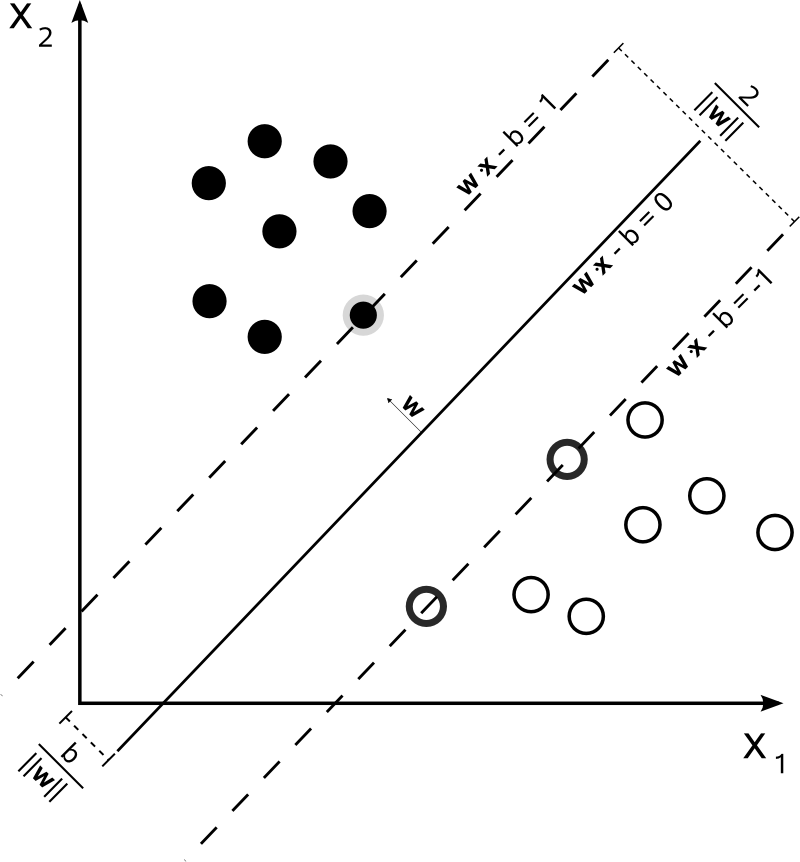
\includegraphics[scale=0.25]{images/svm_vectors}
	\caption{Maximální pás bez bodů trénovací množiny \cite{svm_vectors}}
	\label{fig:svm_vectors}
\end{figure}

\section{Teoretický úvod}

\subsection{Support Vector Machines}
Algoritmy strojového se skládají z \textit{trénovací množiny} a \textit{rozhodovací hranice}. Rozhodovací hranici můžeme též nazývat \textit{hypotéza}. Trénovací množina může obsahovat i správné odpovědi. Algoritmy tedy dělíme na \textit{učení s učitelem} (máme odpovědi) a \textit{učení bez učitele} (nemáme odpovědi).
\\\\
Každý vzorek \textbf{x} trénovací množiny je tvořen množinou příznaků $${x_1,x_2,...x_n},$$kde \textit{n} je počet příznaků. Hypotéza má tvar \textit{h:x->y} což znamená, že hypotéza je zobrazení \textit{x} do \textit{y}. Hypotézu tvoří modelovací parametry $$\Theta_{n},$$které nám umožňují nastavit rozumnou rozhodovací hranici. Jejich hodnoty předem neznáme a získáme je trénováním.

\subsubsection{Lineární rozhodovací hranice}
Metoda strojového učení, která hledá v trénovací množině umístění optimální nadroviny. Tato nadrovina slouží k rozdělení bodů projekce na dvě třídy. V tomto rozdělení je požadováno aby minimum vzdáleností bodů od této nadroviny bylo co největší. Chceme tedy, aby nadrovina měla po obou stranách co nejširší pás bez bodů. K popisu těchto pásů slouží pomocné vektory (\textit{Support Vectors}) (viz Obr.:\ref{fig:svm_vectors}).
\cite{svm_zcu}

\subsubsection{Cenová funkce lineární hranice}
Metoda SVM je vylepšenou verzí \textit{logistické regrese}. Ovšem, na rozdíl od cenové funkce logistické regrese nám SVM nevrací pravděpodobnost, ale rovnou příslušnost klasifikovaného vzorku k třídě 1 nebo 0. Zde vidíme \textit{cenovou funkci} logistické regrese:

$$\min_{\theta} \frac{1}{m}[\sum_{i=1}^{m}y^{(i)}(-\log h_{\theta}(x^{(i)}))+(1-y^{(i)})(-\log(1-h_{\theta}(x^{(i)})))]+\frac{\lambda}{2m}\sum_{j=1}^{n}\theta_{j}^{2}$$

Cenová funkce SVM pak vypadá následovně:

$$\min_{\theta} C \sum_{i=1}^{m}[y^{(i)} Cost_1 (\theta^T x^{(i)})+(1-y^{(i)}) Cost_0 (\theta^T x^{(i)})] + \frac{1}{2} \sum_{j=1}^{n}\theta_{j}^{2},$$

kde \textit{Cost} funkce pro y = 1 je

$$\log\frac{1}{1 + e^{-\Theta^{T}x}}$$

a funkce \textit{Cost} funkce pro y = 0 je

$$\log(1-\frac{1}{1 + e^{-\Theta^{T}x}}).$$

Optimalizací cenové funkce získáme hodnoty parametrů $\Theta$, které určují tvar hypotézy.
\\\\
Hodnota \textit{C} je regularizační faktor, který ovlivňuje výběr hypotézy. Rozumně vybraná hodnota pak umožní dělat ve výběru hypotézy kompromisy v extrémních případech rodělení tříd v trénovací množině:

\begin{enumerate}
	\item C - vysoké = malá odchylka, velký rozptyl (malá $\lambda$), hrozí \textit{overfitting}
	\item C - malé = velká odchylka, malý rozptyl (velká $\lambda$), hrozí \textit{undefitting}
\end{enumerate}

\begin{figure}[!ht]
	\centering
		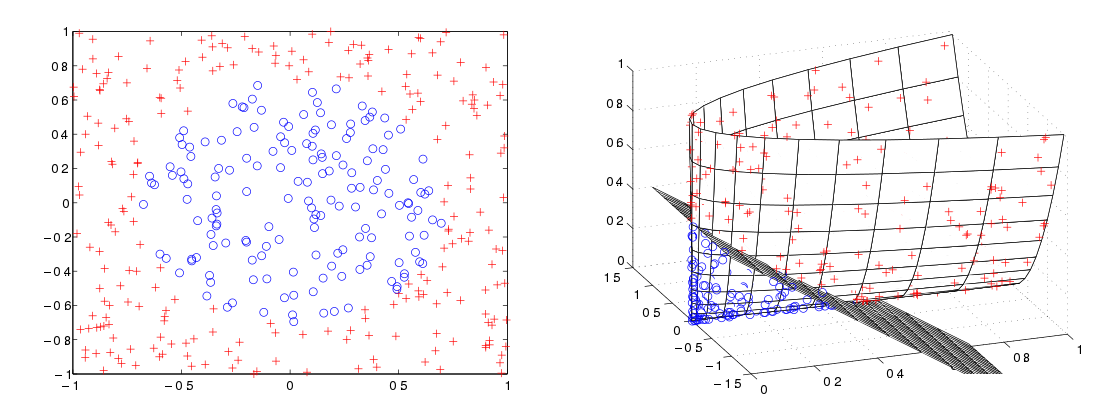
\includegraphics[width=\textwidth]{images/linear_nonlinear}
	\caption{Ukázka lineárně neseparabilních a separabilních dat.\cite{svm_wiki}}
	\label{fig:linear_nonlinear}
\end{figure}

\subsubsection{Nelineární rozhodovací hranice}
Máme-li trénovací množinu, pro kterou je rozhodovací hranice nelineární (viz. Obr.:\ref{fig:linear_nonlinear}), musíme použít metodu jader (\textit{Kernels}). Zavedeme si \textit{i} pomocných bodů tzv. \textit{landmarky}. Každý landmark $l^{(i)}$ nese hodnotu třídy, do které patří. Ke každému prvku $x^{(n)}$ trénovací množiny spočteme podobnost $f_{i}$ s každým landmarkem $l^{(i)}$. Pro každý prvek trénovací množiny tak dostaneme vektor podobnosti $f^{(n)}$. Podobnost počítáme následovně:

$$f_{i}(x^{(n)},l^{(i)}) = exp(-\frac{||x^{(n)} - l^{(i)}||}{2\sigma^2})$$

\noindent vektor podobnosti pak bude vypadat:

$$f^{(n)} = [f_{1},f_{2},f_{3},...,f_{i}]$$

\noindent Jádrem se nazývá funkce počítání podobnosti. V tomto případě je jádro \textit{Gaussové}. Parametr \textit{sigma} nám určuje míru podobnosti. Máme i jiné funkce jádra jako například \textit{Polynomiální} nebo \textit{Lineární}. Lineární jádro je předchozí případ lineárně separabilních dat.\cite{svm_robots},\cite{svm_wiki}

\subsubsection{Cenová funkce nelineární hranice}
Při použití gaussového jádra máme předpočítaný vektor podobnosti pro každý prvek trénovací množiny. To znamená, že vektor podobnosti může reprezentovat daný prvek trénovací množiny. Cenouvou funkci tedy můžeme pozměnit do tvaru:

$$\min_{\theta} C \sum_{i=1}^{m}[y^{(i)} Cost_1 (\theta^T f^{(i)})+(1-y^{(i)}) Cost_0 (\theta^T f^{(i)})] + \frac{1}{2} \sum_{j=1}^{n}\theta_{j}^{2}$$

Pozor, gaussové jádro je citlivé na velké rozdíly hodnot mezi jednotlivými příznaky. Je dobré příznakový vektor nejdříve naškálovat a až poté počítat cenovou funkci.

\subsection{Sequential minimal optimization (SMO)}
???

\section{Implementace}
Výsledný program je naprogramovaný v matematickém jazyce Octave. Tuto variantu jsem zvolil z důvodu velkého množství matematických operací v úloze. Jelikož výsledný program slouží pouze k vyzkoušení dané problematiky, je tento jazyk optimální pro jeho realizaci.
\\\\
Program se spouští v hlavní části \texttt{main.m}. Hlavní část je pak rozdělena na \texttt{settings.m, preprocessing.m}, \texttt{trainManual.m}, \texttt{predictManual.m}, \texttt{statistics.m} a \texttt{evaluateSample.m}.

\subsection{Příprava dat}
Před načtením dat jsem analyzoval jednotlivé příznaky všech prvků trénovací množiny pomocí programu \textit{Weka-3.8.1}.

\subsubsection{Analýza a čištění}

Příprava prostředí, načtení a čištění dat probíhá v částech settings.m a preprocessing.m. Po prozkoumání jednotlivých příznaků jsem zjistil, že sloupce \textit{embarked, cabin} a \textit{age} mají některá pole nevyplněná. V příznaku embarked chybí 2 hodnoty, proto je jednodušší tyto řádku smazat než vymýšlet postup nahrazení. Naopak příznaku cabin chybí 
687 z 891, což je 77\%. Pokud bychom chtěli tyto mezery v datech nahradit například střední hodnotou nebo generátorem náhodných čísel, výsledné zkreslení hypotézy by bylo příliš velké a stala by se tato operace spíše nevýhodou. Proto sloupec cabin odstraníme úplně. Posledním příznakem s chybějícími hodnotami je age. Zde chybí 177 z 891, což je 20\%. To není zase tak mnoho, chybějící hodnoty nahradím střdními hodnotami příznaku. Výslednou hypotézu mi to může zkreslit, ale myslím si že ne tolik, jako by se tomu stalo v případě příznaku cabin.
\\\\
Příznak cabin bych odstranil i z jiného důvodu. Sice obsahuje pouze 147 hodnot, ale z toho je 101 unikátních. Pokud mám velké množství unikátních hodnot, výsledný sloupec mi poté slouží jako množina identifikátorů. Identifikátory do trénovací množiny nepřináší žádnou přidanou hodnotu a jsou tudíž zbytečné. Odstraním tedy i sloupec name, který je jednoznačným identifikátorem, protože má 100\% unikátních hodnot.

\subsubsection{Konverze}
Jelikož nejsou všechny příznaky číselné hodnoty, je nutné je konvertovat. Patří sem sloupce age, ticket a embarked. U sloupců ticket a embarked nevím, jaké jiné hodnoty se zde mohou vyskytovat, takže převod na určitou řadu čísel zde nejde použít. Znaky každé buňky tedy převedu podle \texttt{ASCII} tabulky na znaky a sečtu. Náhled konverze pro sloupec embraked:

\begin{lstlisting}
# preprocessing.m
# line 43 
# EMBARKED to NUMBER
for i = 1:countRow
  data(i, 8) = sum(cell2mat (toascii(data(i, 8))));
endfor
\end{lstlisting}

\noindent Příznak sex lze konertovat tak, aby jsme z toho dostaly lepší hodnotu. Jelikož víme, že pohlaví u lidí jsou pouze dvě, převedeme hodnoty \texttt{male} a \texttt{female} na binární klasifikaci, tedy hodnoty 0 a 1. Převod vypadá následovně:

\begin{lstlisting}
# preprocessing.m
# line 26 
# Convert MALE/FEMALE to BINARY
for i = 1:countRow
  if (strcmpi(data(i, 2), 'female'))
    data(i, 2) = 1;
  else
    data(i, 2) = 0;
  endif
endfor
\end{lstlisting}

\subsection{Trénování}
\subsubsection{Škálování a matice podobnosti}
Před trénováním jsou data ještě škálována aby se srazili rozdíly mezi jednotlivými příznaky a došlo tak ke správnému natrénování. Příznaky se škálují odečtením maxima příznaku přes všechny vzorky trénovací množiny.

$$
s_{n}^{i} = x_{n}^{i} - \max_{i} x_{n} \,;\, i \in <1;m>
$$

\noindent Kód škálování pak vypadá následovně:

\begin{lstlisting}
# scale.m
# line 7 
for i = 1:countColumn
  for j = 1:countRow
    scaledTrainingSet(j,i) = trainingSet(j,i) / maxFeature(i);
  endfor
endfor 
\end{lstlisting}

\noindent Před začátkem trénování vytvořím matici podobnosti $f$. Jako landmarky označím všechny prvky trénovací množiny. Matice podobnosti tedy bude obsahovat podobnost všech prvků trénovací množiny vůči ostatním prvkům. Matice $f$ bude symetrická. Kód pro výpočet podobnosti je kód gaussového jádra.

\begin{lstlisting}
# gaussianKernel.m
# line 5
function f = gaussianKernel(x1, x2, sigma)
  f = exp(-norm(x1 - x2)^2 / 2 * sigma^2); 
end
\end{lstlisting}

\subsubsection{Minimalizace cenové funkce}
Samotné trénování probíhá v části \texttt{trainManual.m}.
???

\newpage

\section{Závěr}

\section{Uživatelská příručka}
\subsubsection{Požadavky}
Aby bylo možné program spustit, je nutné mít nainstalovaný program GNU Octave ve verzi 4.2.0.

\subsubsection{Načtení dat}
Program na načítá data ze souboru \textit{.csv}. Počítá také s tím, že data jsou ve stejné složce jako všechny potřebné moduly programu (*.m). Pokud jsou tedy data uloženy jinde, je nutné změnit cestu k souboru v modulu \texttt{settings.m} na řádce 25.

\begin{lstlisting}
# settings.m
# line 25
data = csv2cell('titanic.csv');
\end{lstlisting}

\begin{figure}[!ht]
	\centering
		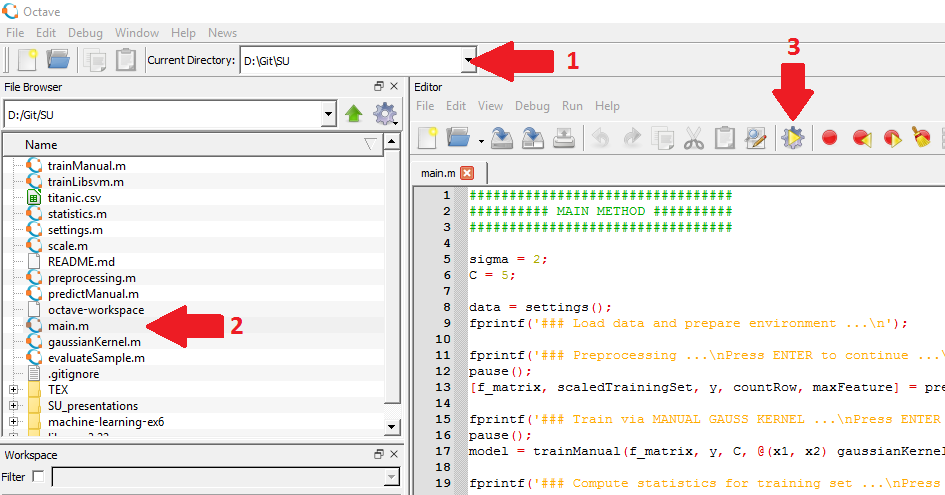
\includegraphics[width=\textwidth]{images/runWithGUI}
	\caption{1. Nastavení cesty do složky programu, 2. Hlavní program (rozkliknout do záložky), 3. Spuštění programu}
	\label{fig:runWithGUI}
\end{figure}

\subsubsection{Spuštění}
Máme dvě možnosti spuštění:

\begin{enumerate}
	\item - Octave (GUI) : Máme-li Octave ve verzi s GUI, tak po spuštění programu navedeme Octave do správné složky s programem a spustíme modul \texttt{main.m} (viz Obr.:\ref{fig:runWithGUI})
	\item - Octave (CLI) : Spouštíte-li Octave v příkazové řádce, je nutné se přesunout do složky programu s moduly a zadat pouze příkaz \texttt{main} (viz Obr.:\ref{fig:runWithoutGUI}.
\end{enumerate}

\begin{figure}[!ht]
	\centering
		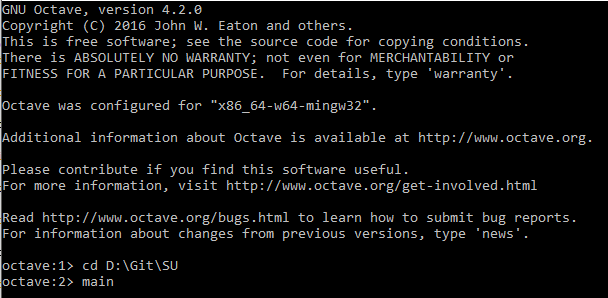
\includegraphics[width=\textwidth]{images/runWithoutGUI}
	\caption{Spuštění Octave (CLI)}
	\label{fig:runWithoutGUI}
\end{figure}

Dále už průběh pokračuje v obou prostředí stejně. Uživatel stiskem klávesy \texttt{ENTER} načtení a úpravu dat. Jakmile jsou data připravena, spustí se výpočet matice podobnosti indikovaný hláškou \texttt{Similarity ...}. Dokončení výpočtu je značeno hláškou \texttt{... Done!}. Následovně je uživatel vyzván k potvrzení trénování hypotézy. Chvilku se nic neděje, protože se matice podobnosti vektorizuje. Trénování začíná v okamžiku vyskočení hlášky \texttt{Training ...} a dokončení opět poznáme přes \texttt{... Done!}.
\\\\
Program tedy přejde k výpočtu statistik a zobrazí uživatel v procentech, jak moc hypotéza natrénovaná pomocí křížové validace.

\section{Testování}

\appendix
\begin{thebibliography}{99}

\bibitem{svm_zcu}
EKŠTEIN, Kamil. \textit{Support Vector Machines} [online]. Plzeň, 2012 [cit. 2017-01-31]. Dostupné z: \url{https://portal.zcu.cz/CoursewarePortlets2/DownloadDokumentu?id=123920}. Přednášky k předmětu Strojové učení. Západočeská univerzita v Plzni.

\bibitem{andrew}
NG, Andrew. \textit{CS229 Lecture notes - SVM} [online]. Standford, 2016 [cit. 2017-01-31]. Dostupné z: \url{http://cs229.stanford.edu/notes/cs229-notes3.pdf}. Přednášky k předmětu Machine Learning - CS229. Stanford University.

\bibitem{andrew}
NG, Andrew. \textit{Support Vector Machines} [online]. Standford, 2016 [cit. 2017-01-31]. Dostupné z: \url{https://d3c33hcgiwev3.cloudfront.net/_246c2a4e4c249f94c895f607ea1e6407_Lecture12.pdf?Expires=1485993600&Signature=MGhCSj6vnfSMVWpDERGUz8fc2312duxtjEpe2o4R0vhRA9KQQuPnZOPulQy5I0mCrICpxj3M0efelTXkmFFQsKB8VaVCYc0v7qPGH1pnWnL6WdQ1CEkpGAu~i3NfLItowu0Ge3C885eDXuSYBGmDGLUh83obXuukWx9ALN6J5yQ_&Key-Pair-Id=APKAJLTNE6QMUY6HBC5A}. Přednášky k předmětu Machine Learning. Stanford University.

\bibitem{svm_wiki}
Support vector machine. In: \textit{Wikipedia: the free encyclopedia} [online]. San Francisco (CA): Wikimedia Foundation, 2016 [cit. 2017-01-31]. Dostupné z: \url{https://cs.wikipedia.org/wiki/Support_vector_machines}.

\bibitem{svm_robots}
ZISSERMAN, Andrew. In: \textit{SVM dual, kernels and regression} [online]. Oxford, 2015 [cit. 2017-01-31]. Dostupné z: \url{http://www.robots.ox.ac.uk/~az/lectures/ml/lect3.pdf}.

\end{thebibliography}

\end{document}
